\documentclass{article}
\usepackage{log_2022}   % for anonymous submission
% \usepackage{log_2022}         % for camera-ready version
% \usepackage[preprint]{log_2022}
%                               % for preprint version
% \usepackage[eatrack]{log_2022}
%                               % for accepted extended abstracts

\usepackage{booktabs}           % professional-quality tables
\usepackage{multirow}           % tabular cells spanning multiple rows
\usepackage{multicol}
\usepackage{amsfonts}           % blackboard math symbols
\usepackage{graphicx}           % figures
\usepackage{duckuments}         % sample images
\usepackage{array}
\usepackage{lipsum}
\usepackage{subcaption}
\usepackage{wrapfig}


\usepackage[utf8]{inputenc} % allow utf-8 input
\usepackage[T1]{fontenc}    % use 8-bit T1 fonts
\usepackage{url}            % simple URL typesetting
\usepackage{nicefrac}       % compact symbols for 1/2, etc.
\usepackage{microtype}      % microtypography

% If you want to use natbib:
\usepackage[numbers,compress,sort]{natbib}
%                               % for numerical citations
% \usepackage[sort,round]{natbib}
%                               % for textual citations

% If you want to use bibLaTeX:
% \usepackage[
%      backend=biber,
%      style=numeric-comp,
%      backref=true,
%      natbib=true]{biblatex}
% \addbibresource{reference.bib}

\usepackage[mathscr]{euscript}
\usepackage[export]{adjustbox}

\newcommand{\rex}[1]{{{\textcolor{magenta}{[rex: #1]}}}}
\newcommand{\jure}[1]{{{\textcolor{red}{[Jure: #1]}}}}
\newcommand{\michal}[1]{{{\textcolor{blue}{[Michal: #1]}}}}

\newcommand{\update}[1]{{{\textcolor{ForestGreen}{[Update: #1]}}}}

\usepackage{enumitem}
\newcommand{\etal}{\textit{et al.}\xspace}
\newcommand{\alg}{\textsc{PHIL}\xspace}
\newcommand{\sail}[0]{\textsc{SaIL}\xspace}


\usepackage[ruled,vlined]{algorithm2e}  %updated version of algorithm2e.sty is in ./ folder.
\SetKwComment{Comment}{$\triangleright$\ }{}
\newcommand{\algorithmStyle}[0]{\footnotesize}
\usepackage{amsmath,amssymb}

\DeclareRobustCommand{\bbone}{\text{\usefont{U}{bbold}{m}{n}1}}
\DeclareMathOperator{\EX}{\mathbb{E}} % expected value
\newcommand{\VS}{\mathcal{V}}
\newcommand{\xhdr}[1]{{\noindent\bfseries #1}.}


\title[Submission Guidelines and Formatting Instructions for LoG Conference 2022]{Learning Graph Search Heuristics}

\begin{document}


\appendix
\newpage

\section{Discussion, Limitations, and Future Work}
\label{sec:future-work}


\paragraph{Injection from nodes and edges to features}  As mentioned in Section \ref{sec:experiments-diversity}, if multiple graph nodes or edges have the same features, our heuristic learning method is challenging to apply. To ensure that \phil has a constant time complexity, we bound the number of neighbouring nodes used for graph convolutions around new fringe nodes, and do not perform any graph convolutions on goal nodes. However, if multiple graph nodes have the same features, or they perhaps do not have any features at all, we may need to perform operations that are not constant in the size of the graph, such as sampling anchor nodes as in position-aware GNN \cite{you2019position}, or collecting more expressive Node2Vec \cite{grover2016node2vec} style features. Since the time complexity of these methods are relatively high (e.g. position-aware GNN's time complexity is $O(|V|^2\log^2|V|)$ while the Dijkstra algorithm only runs in $O(|V|\log|V| + |E|)$), we do not use them unless necessary. For use cases where injections from nodes \& edges to features are hard to guarantee, we encourage practitioners to increase $n$ or potentially perform multiple convolutions on fringe and goal nodes.

\paragraph{Restricted fringe evaluation} As explained in Section \ref{sec:approach}, \phil only evaluates new fringe nodes which are obtained after expanding a node. In practice, this means that once \phil assigns a heuristic value to a node, the value is never updated. While this approach is favorable in terms of the time-complexity of heuristic computations, it does not allow \phil to re-evaluate potentially promising nodes for expansion, based on its updated belief about the POMDP state. We believe that methods that predict the features of promising nodes to expand combined with locality-sensitive hashing or approaches that incorporate node value uncertainty present promising avenues for future work.

\paragraph{Solutions not necessarily optimal} For a best-first search algorithm to find optimal solutions, the used heuristics needs to be \textit{admissible} \cite{russell2002artificial}. In our approach, we do not guarantee the trained heuristics to be \text it{admissible}, which means that when combined with best-first search, \phil would not guarantee optimal final solutions. On the other hand, our approach is concerned with finding \textit{satisficing} solutions as quickly as possible, which is motivated by possible applications in Section \ref{sec:intro}. As in \cite{bhardwaj2017learning}, our learned heuristics can be easily incorporated into a framework such as multi-heuristic A* \cite{aine2016multi}, where any number of inadmissible heuristics can be used with a single admissible heuristic, and the final solution cost sub-optimality is bounded.  An interesting avenue for future work would be to design heuristic learning loss functions that discourage models from over-estimating heuristic values.

\paragraph{Full memory permutation invariance} As noted in Section \ref{sec:approach}, our memory module is invariant to the permutation of nodes in $\VS_{new}$. However, due to how the $\textsc{GRU}$ module is applied, we do not guarantee that that the memory is permutation invariant with respect to the sequence in which nodes are expanded, or equivalently the sequence of $\VS_{new}$ sets. It could be desirable to guarantee such permutation invariance, as the observations are still nodes and edges of a graph, which may not contain sequential inductive biases. Recent work by Cohen \etal \cite{cohen2020regularizing} shows that a simple regularization trick can help efficiently train permutation invariant RNNs. It would be interesting to explore in which cases does full permutation invariance improve \phil's performance.  


\paragraph{Directed graphs} As one may notice, most of the examples in this work include graphs that are undirected. The main reason for this is that once we have directed edges in a graph, it may happen that a particular node does not have a path toward the goal, which means that the oracle cost would be effectively undefined. One option for avoiding this issue is adding parallel backward edges during training, ensuring that paths to goals always exist (assuming that the start and goal nodes are parts of the same connected component). This way, \phil is correspondingly penalised for expanding a node that does not immediately lie on a path to the goal.

\paragraph{Ethical considerations} Search algorithms with heuristics can be used within unethical systems. However, our work is not tailored for any particular use cases, and hence we do not believe that it has clear direct negative consequences.

\section{Practical implementation details}

As noted in our abstract, at test time, the heuristic function obtained from \phil can be directly used as a heuristic in an algorithm such as A* or greedy best-first search. In practice, this means that we maintain a priority queue of nodes and distances predicted by the \phil heuristic and greedily expand the nodes which are predicted to be closest to the goal, as seen in Figure \ref{fig:implementation}.

To ensure fast training in Algorithm \ref{alg:il_alg}, we maintain two priority queues, one for \phil and one for the oracle heuristic. On every expansion, we update both the \phil queue and oracle queue. This way, probabilistically blending the two greedy policies comes down to either popping from the \phil queue or the oracle queue.

\begin{figure}[htpb]
\centering
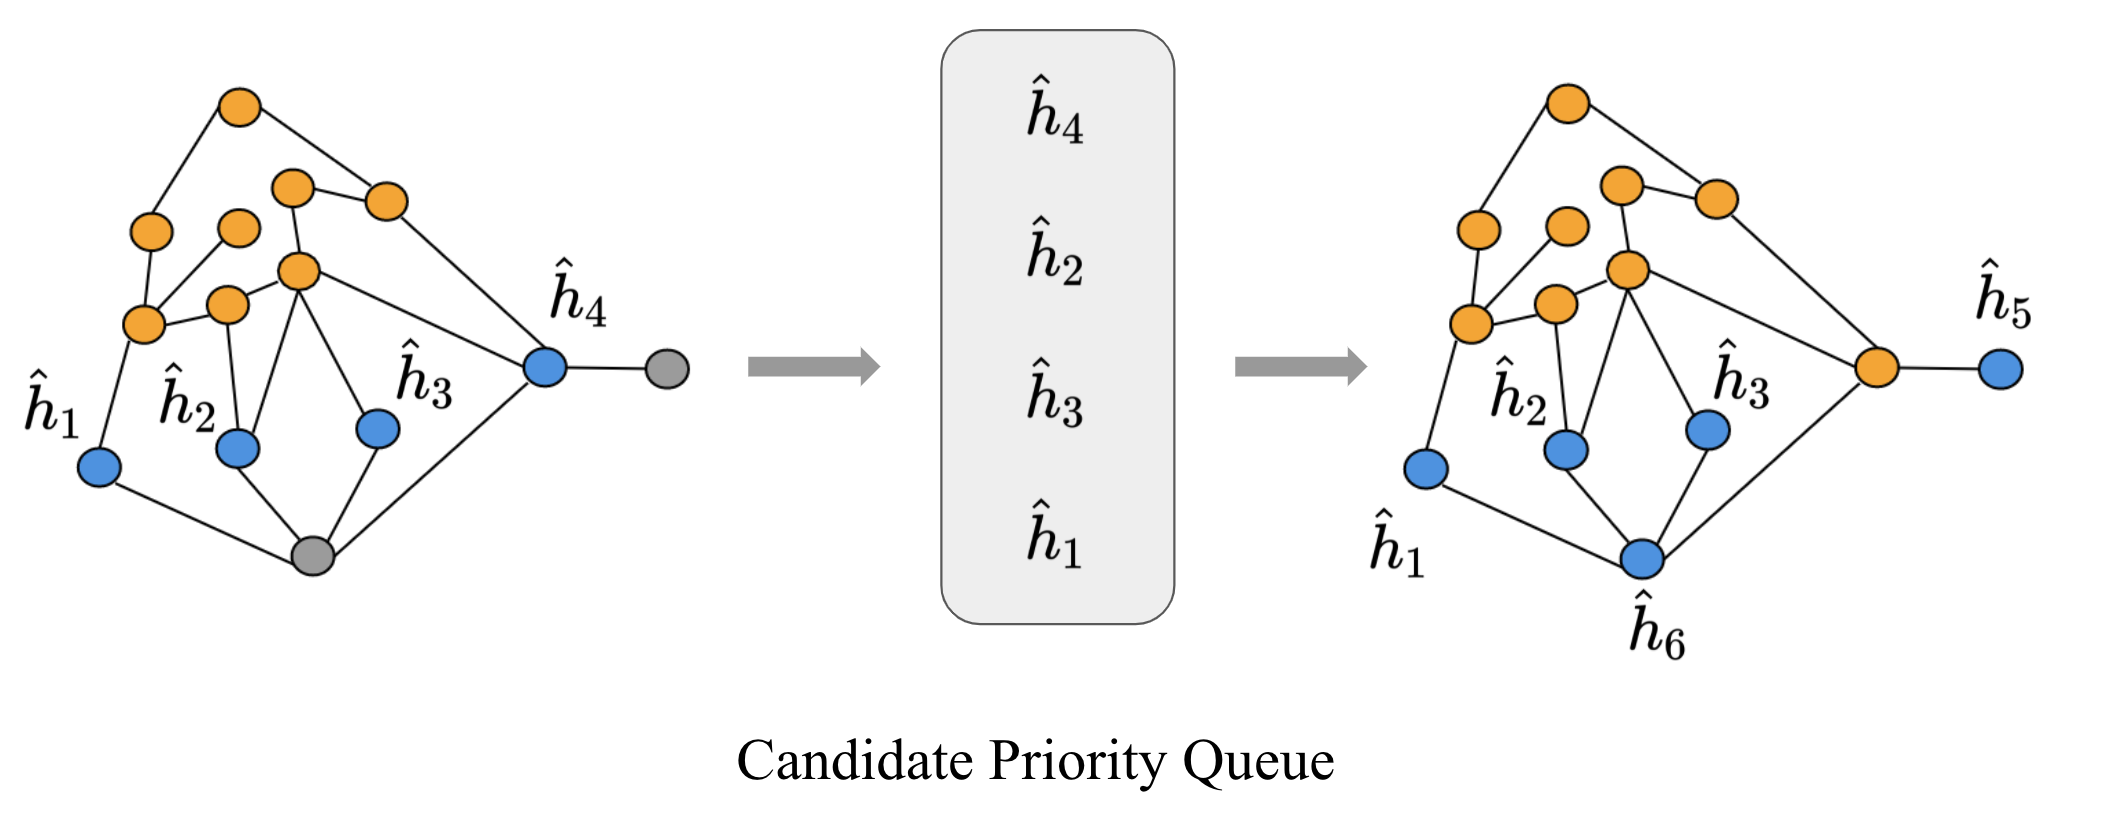
\includegraphics[width=0.7\textwidth]{figures/pqueue.png}
\caption{PHIL is used as a heuristic to predict the distances of each node, similarly as a heuristic function in best-first search. This figure illustrates a single queue `pop' operation.}
\label{fig:implementation}
\end{figure}

\section{Training, Baselines, Hyperparameters, and Datasets}
\label{sec:baselines-and-datasets}
\paragraph{Baselines} In our experiments we use a range of both \textit{learning-based} and \textit{classical} \textit{baselines}. Our \textit{baselines} include:

\begin{itemize}
    \item \textbf{Neural A*} \cite{yonetani2020path}: Neural A* learns a differentiable version of A* search on two-dimensional grid graphs. It cannot be straightforwardly adapted to general graphs, which is why we use it as a baseline solely in Section 5.1.
    
    \item \textbf{\sail} \cite{bhardwaj2017learning}: Imitation learning-based approach for learning search heuristics on grid graphs. \sail is adapted in Section 5.2 to not include robotics domain specific features presented in \cite{bhardwaj2017learning}, as these are not possible to compute for general graphs.
    
    \item \textbf{Supervised Learning} (SL): An $\textsc{MLP}$ trained to predict distances between nodes conditioned on node features. In Sections \ref{sec:experiments-diversity}, Sections \ref{sec:experiments-drone} the nodes are sampled from the graph uniformly at random. In Section \ref{sec:experiments-grids}, an oracle policy is rolled out, and data points are collected by sampling random actions during the roll-out as in \sail. This is because in Section \ref{sec:experiments-grids}, the start-goal distribution is not uniform.
    
    \item \textbf{Deep Q Learning}  (QL) \cite{mnih2013playing}: A DQN agent trained to explore the graphs such that $|\VS_{seen}|$ is minimized. The agent receives a negative reward of $-1$ until the goal node is reached in each episode. 
    
    \item \textbf{Cross Entropy Method - Evolutionary Strategies} (CEM) \cite{de2005tutorial}: Derivative free optimization of $h_{\theta}$ using evolutionary strategies. As explained in \cite{bhardwaj2017learning}, the initial population of policies is sampled using a batch size of $40$. Then, each policy is evaluated on $5$ graphs and assigned a score based on the number of expanded nodes for the fitness function. After computing the fitness function, $20\%$ of best-performing policies are selected to be a part of the next population.
    
    \item \textbf{Best-first width search (BFWS)} \cite{lipovetzky2017best}: BFWS adapts greedy best-first search with a generic search history-based novelty metric, which allows it to escape search plateaus and explore relevant nodes. We implement BFWS in experiments from Section 5.1 and 5.3. In Section 5.2, we extend BFWS with boundary-extension features \cite{teichteil2021boundary}, which allows us to apply it to continuous feature spaces. 
    
    \item \textbf{Multi-heuristic A*} (MHA*)\cite{aine2016multi}: Multi-heuristic A* using the Euclidean, Manhattan, and $d_{obs}$ heuristics in a round-robin fashion, where $d_{obs}$ is the distance of the closest uncovered obstacle for a given node.  This baseline is only used in Section \ref{sec:experiments-grids}, where all of these heuristics are well-defined.
    
    \item \textbf{A* search} (A*): A* search algorithm using a Euclidean heuristic function on the node features.
    
    \item \textbf{Greedy best-first search} ($h_{man}, h_{euc}$): Greedy best-first search using Manhattan and Euclidean heuristics, respectively.
    
    \item \textbf{Breadth-first-search} (BFS): Vanilla breadth-first-search without any heuristic.
\end{itemize}


\xhdr{Datasets} Here, we provide more details about the datasets used in Section \ref{sec:experiments-diversity} and Section \ref{sec:experiments-drone}. For more information about datasets used in Section \ref{sec:experiments-grids}, we refer the reader to Bhardwaj and Choudhury \etal \cite{bhardwaj2017learning}. 


In our experiments using diverse graphs, as noted in Section \ref{sec:experiments-diversity}, we use the node \& edge features provided in each dataset for training and testing. The three exceptions to this are the PPI, OSMnx datasets, and citation networks. As discussed in Appendix A, we added node labels (i.e., $120$ dimensional label vectors) as features in the PPI dataset because the default node features were not unique. In the OSMnx networks, we did not use all the provided node and edge features, rather only the geographical node coordinates. We further augmented the OSMnx node features with their degree centrality and included Laplacian, modularity, and Bethe Hessian edge features. For citation networks, we only used the first $128$ features to make the search problem more challenging.

In static graphs (such as the OSMnx networks), it may be helpful to augment the graph with expressive features that could be useful for heuristic computations, such as eigenvectors of the graph Laplacian matrix. In non-static graphs, these operations would typically be too expensive to re-compute on each pathfinding attempt. Note that computing more expressive features such as betweenness or percolation centrality have higher time complexities than computing shortest path distances between all pairs of nodes. Due to their time complexity, these features are impractical pre-compute, though they would likely lead to superior search heuristics.


In Section \ref{sec:experiments-drone},  we built our environment using the CoppeliaSim simulator \cite{coppeliaSim}, and the Ivy framework by Lenton \etal \cite{lenton2021ivy}. Figure \ref{fig:rooms} presents the environments which we refer to as \textit{room adversarial} and \textit{room simple} in Table \ref{tab:table-3}. The \textit{room simple} environment is equivalent to the Ivy drone demo environment --- a single room with a table surrounded by chairs in the middle of the room and various furniture close to the walls. The main difference between \textit{room simple} and \textit{room adversarial} is that \textit{room simple} only contains a single table in the middle of the room. In contrast, in \textit{room} \textit{adversarial}, three tables span to a wall, this was creating a bottleneck for naive heuristics. Note that the drones are not allowed to fly under furniture to make the environment more challenging.

\begin{figure}[!htb]
    \centering
    \begin{minipage}{.4\textwidth}
        \centering
        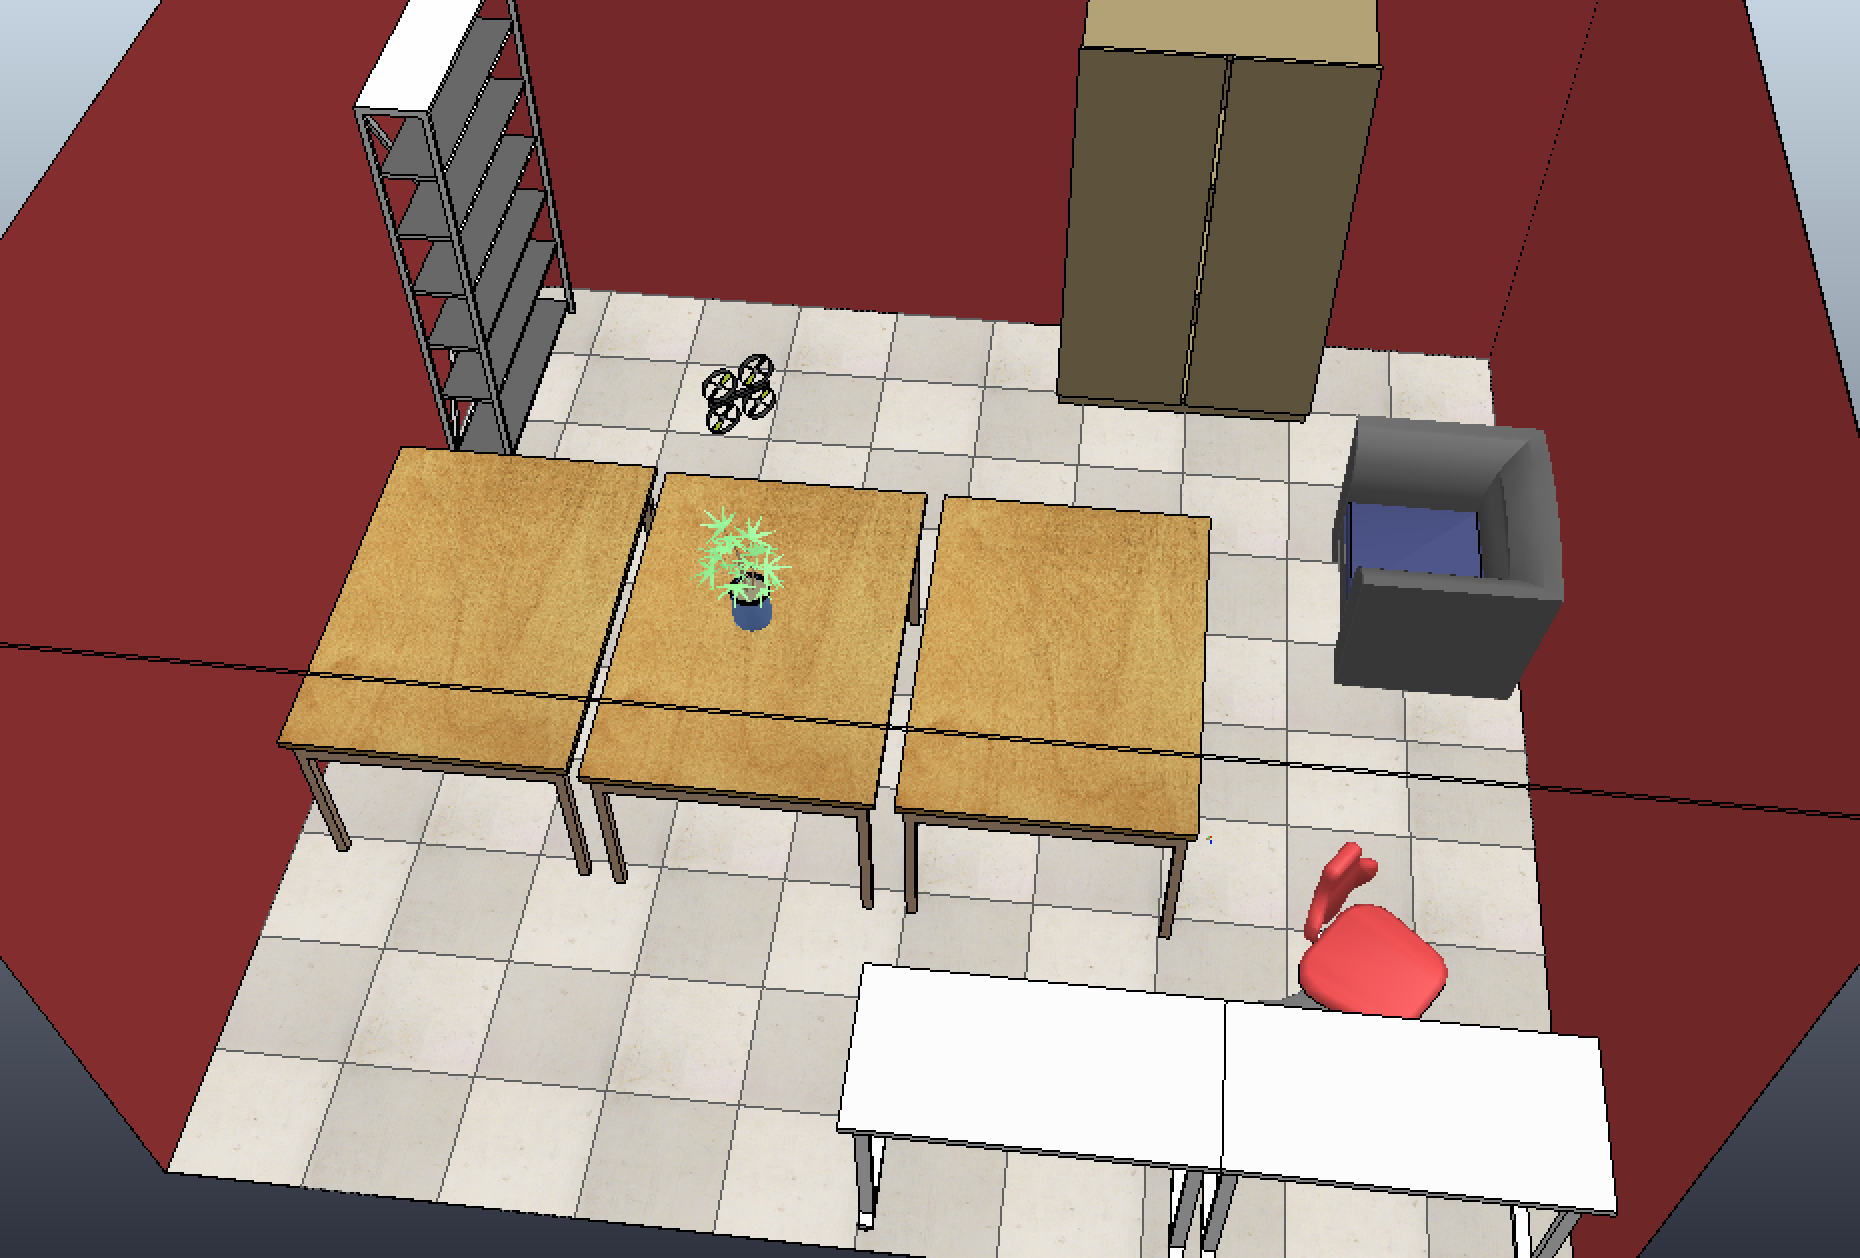
\includegraphics[width=0.8\linewidth, height=0.15\textheight]{figures/adv.png}
    \end{minipage}%
    \begin{minipage}{0.4\textwidth}
        \centering
        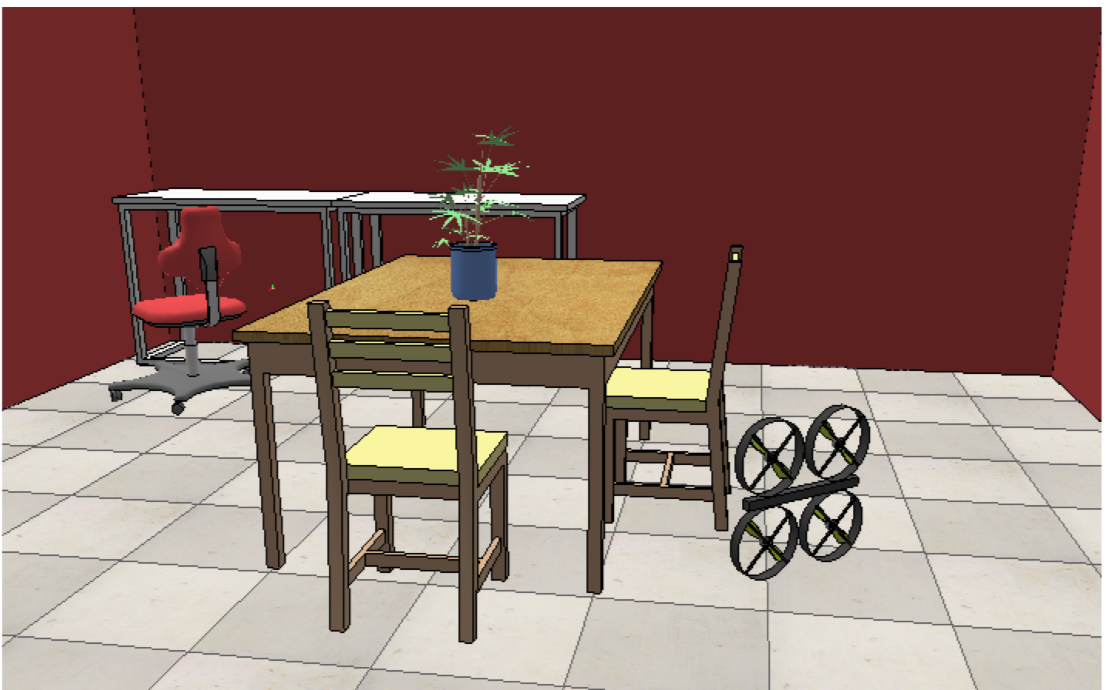
\includegraphics[width=0.8\linewidth, height=0.15\textheight]{figures/simple.png}
    \end{minipage}

\caption{We present two CoppeliaSim environments used for our UAV flight experiments. On the left, we have the \textit{adversarial room environment}, on the right, we present the \textit{room simple} environment.}
\label{fig:rooms}
\end{figure}



\paragraph{Hyperparameters in diverse graphs} With regards to the diverse graph experiments (Section \ref{sec:experiments-diversity}), there are in-practice three parameters that we can tune for each dataset: $n$, $t_\tau$ $T$. Recall that the hyperparameter $n$ is the maximal size of the 1-hop neighborhood around the new fringe nodes sampled during training. We found that a rule of thumb of setting $n$ to the minimum of $8$ and the average node degree in the given graph dataset worked reasonably well. In practice, $n$ should be tuned to optimize the search effort \& wall-clock performance trade-off. In terms of $T$, it is advisable to set it such that the algorithm can reach target nodes during training. Hence, we found that setting $T$ roughly to the largest graph diameter is a suitable choice. In terms of $t_\tau$, we train each sequence using the stored old rolled-in states, and for larger graphs ($>10,000$ nodes), we use $t_\tau = 128$, while for smaller graphs (between $10,000$ and $5,000$ nodes), we use $t_\tau = 64$, and otherwise we use a rule of thumb of taking $t_\tau \approx T * 0.2$.

\paragraph{Grid graphs \& drone flight hyperparameters} In our grid graph experiments (Section \ref{sec:experiments-grids}), we use $T = 256$,  $t_{\tau} = 32$, $\beta_{0} = 0.7$, $n = 8$. Finally, in our drone flight experiments, we use the same configuration as in the grid graph experiments. The only differences are that we set $n = 4$,  $t_{\tau} = 64$, and we randomize start and goal nodes both during training and testing.

\paragraph{Optimization} \phil is generally trained using the Adam optimizer with a learning rate of $0.001$ and a batch size of $32$. Once we sample $t \sim \mathcal{U}(0, \dots, T-t_\tau)$ for a roll-in, it can happen that the target is reached in less than $t + t_\tau$ steps. In such cases, we continue the sequence until we reach $t_\tau$ steps or all the graph nodes are explored, in which case we end the episode. Another approach would be to end episodes once the goal node is reached. In practice, we did not find significant performance differences between the two methods.

\section{Ablation studies}
\label{sec:ablation}
For the ablation studies, we use three, $4$-connected versions of down-scaled datasets provided in Bhardwaj \etal \cite{bhardwaj2017learning}: \textit{Gaps+Forest}, \textit{Forest}, and \textit{Alternating gaps}. We downscale each dataset $5\times$, to dimensions $40 \times 40$. While the \textit{Gaps+Forest} dataset presents a more challenging environment with multiple planning bottlenecks and obstacles, \textit{Forest} and \textit{Alternating gaps} are simpler environments with more straightforward heuristics. Figure \ref{fig:envs} present example graphs from the down-scaled datasets \textit{Gaps+Forest}, \textit{Forest}, and \textit{Alternating gaps}.


\begin{figure}[!htb]
\minipage{0.32\textwidth}
  \centering
  \frame{
\includegraphics[width=0.4\linewidth]{figures/ex_0.png}}
\endminipage\hfill
\minipage{0.32\textwidth}
  \centering
  \frame{
\includegraphics[width=0.4\linewidth]{figures/ex_1.png}}
\endminipage\hfill
\minipage{0.32\textwidth}%
  \centering
  \frame{
\includegraphics[width=0.4\linewidth]{figures/ex_2.png}}
\endminipage

\caption{This figure presents the down-scaled datasets used for the ablation experiments. We have \textit{Gaps+Forest} (left), \textit{Forest} (centre), and \textit{Alternating gaps} (right).}
\label{fig:envs}
\end{figure}

In each ablation experiment, unless stated otherwise, we use a batch size of $8$, the Adam optimizer with a learning rate of $0.01$, and up to $20$ roll-in steps. The $\textsc{MLP}$ in \phil has $3$ layers of width $128$, \textit{LeakyReLU} activations, and the memory state has $d=64$ dimensions. 2D grid coordinates are used as node features, similarly as in Section \ref{sec:experiments-grids}. We report the number of explored nodes with respect to A* or with respect to the optimal number of expansions (i.e., the shortest path distances between nodes). All experiments are performed across $3$ random seeds, and standard deviations are used for error bars.

\subsection{Zeroed-out states vs. Rolled-in states}
\label{sec:zeronero}

There is a trade-off between using rolled-in states for downstream training using backpropagation through time (i.e., storing $z_t$ after each roll-in) and using zeroed-out states (i.e., storing zeroed-out initial states). Namely, past rolled-in states $z_t$ are out-of-distribution for optimized versions of $h_\theta$, but \phil may use these embeddings for inferring initial node distances because $z_t$ contains information about the rolled-in graph. On the other hand, zeroed-out states are always in-distribution for $h_\theta$, but the algorithm is constrained to start from an initial state of $\vec{\mathbf{0}}$ in regions where this may never be the case at test time. Our goal is to gain insight into when one method is preferable over to the other in this ablation.

\begin{figure}[htpb]
\centering
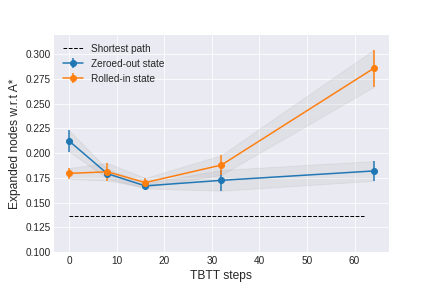
\includegraphics[width=0.6\textwidth]{figures/zero_nero2.png}
\caption{This plot illustrates the performance of \phil with zeroed-out initial states vs. stored rolled-in initial states during training across multiple TBTT steps.}
\label{fig:rolled-vs-zero}
\end{figure}


We train two versions of \phil, one with zeroed-out initial states for TBTT on each trajectory (\phil-zero), and one with initial states stored from roll-ins of the past versions of \phil (\phil-roll). Both versions are trained for $t_\tau = 0, 8, 16, 32, 64$ TBTT steps using the \textit{Gaps+Forest} graph dataset. Figure \ref{fig:rolled-vs-zero} illustrates the performance progress across TBTT steps of both of these approaches. Firstly, we observe that up to around $t_\tau = 16$ steps; both approaches positively benefit from performing more backpropagation steps through time, reinforcing that the memory module brings overall performance benefits. Further, we may see the performance difference of \phil-roll and \phil-zero at $0$ steps. In this region, \phil-roll outperforms \phil-zero by about $3\%$, which is following the intuition of the rolled-in states containing useful information about the embeddings of rolled-in graphs. Secondly, we can notice that the performance of \phil-zero plateaus after $16$ steps. This plateau suggests that the graph may not contain useful information for inferring node distances beyond $16$ backpropagated steps. Finally, the performance of \phil-roll decreases much steeper than that of \phil-zero once it starts deteriorating after $16$ steps, which could mean that there is some form of error compounding once \phil makes predictions from a wrongly initialised state during training.

\paragraph{Conclusion} The main takeaway of this ablation experiment is that if one would like to perform only a few TBTT steps (i.e., low $t_\tau$), using rolled-in states will likely provide some performance benefits. On the other hand, as  $t_\tau$ increases, it is preferable to use zeroed-out initial states. Practitioners can determine this choice on a per-problem basis.


\subsection{Effect of GNN choice} 

In this ablation we assess what effects do different graph neural networks have on the performance of \phil. Namely, we train the \phil-zero from the previous ablation, using $t_\tau = 16$, $n=4$ and five different GNNs: GAT (Veličković \etal \cite{velivckovic2017graph}), MPNN (\textit{max}), MPNN (\textit{sum}) (Gilmer \etal \cite{gilmer2017neural}), DeeperGCN (\textit{softmax}), and DeeperGCN (\textit{power}) (Li \etal \cite{li2020deepergcn}). We report the ratio of explored nodes with respect to A* in Table \ref{tab:table-4}.

\begin{table*}[!htb]
\centering
\resizebox{0.7\columnwidth}{!}{%

\begin{tabular}{cccc} \toprule
 \textbf{GNN}   & \textbf{Alternating gaps} & \textbf{Forest} & \textbf{Gaps+Forest} \\ \midrule
GAT   & 0.077 ± 0.0110 & 0.065 ± 0.0013  & \textbf{0.154 ± 0.0112} \\ 
MPNN (\textit{max})   & 0.071 ± 0.0834 & \textbf{0.064 ± 0.0004}  & 0.158 ± 0.0143  \\ 
MPNN (\textit{sum})   & 0.095 ± 0.0487 & 0.07 ± 0.0085  & 0.187 ± 0.0135  \\ 
DeeperGCN (\textit{softmax})   & \textbf{0.069 ± 0.0008} & \textbf{0.064 ± 0.0030}  & 0.164 ± 0.0113 \\ 
DeeperGCN (\textit{power})  & 0.076 ± 0.0027 & 0.07 ± 0.0101  & 0.19 ± 0.0037   \\ \bottomrule
\end{tabular}
}
\caption{This table presents the results obtained using different graph convolutions in the three graph datasets from the ablation study. We can observe that maximisation-based aggregation performs better on average, while attention can provide performance benefits in the challenging \textit{Gaps+Forest} graphs.}
\label{tab:table-4}
\end{table*}


\begin{wrapfigure}[13]{r}{0.4\textwidth}
  \centering
  
\includegraphics[width=0.5\linewidth]{figures/optimal_staregy.png}
    \caption{This figure illustrates \phil using the DeeperGCN (\textit{softmax}) GNN learning the optimal heuristic strategy in the \textit{Alternating gaps} dataset.}
  \label{fig:optimal-strategy}
\end{wrapfigure}



In general, we find that maximisation-based aggregation approaches tend to perform better than other approaches by $1.57 \%$ on average. Note that this comparison only includes the MPNN and DeeperGCN GNNs. DeeperGCN (\textit{softmax}) achieves the best results on both the \textit{Alternating gaps} and \textit{Forest} datasets. Further, using DeeperGCN (\textit{softmax}), \phil learned the optimal strategy for finding the goal in the \textit{Alternating gaps} dataset, which is to follow the path along the bottleneck wall, as seen in Figure \ref{fig:optimal-strategy}.



GAT outperforms other approaches on the \textit{Gaps+Forest} dataset, which is also the most complex of the three datasets. This finding suggests that forms of attention could be useful for learning heuristics in more complex graphs. In Figure \ref{fig:figure-3convs}, we can see a side-by-side comparison of GAT, DeeperGCN (\textit{softmax}), and MPNN (\textit{sum}) in the \textit{Gaps+Forest} graph dataset. We may observe that the GAT-based and DeeperGCN-based heuristics find strategies that are close to optimal, while MPNN (\textit{sum}) performs a similar strategy, but with slightly more expansions.

\begin{figure}[htp]

\centering
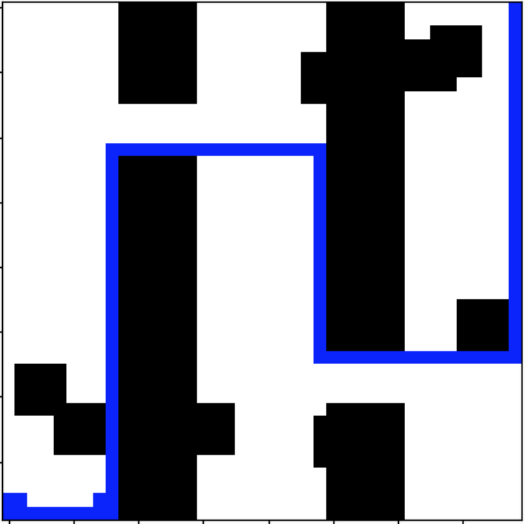
\includegraphics[width=.2\textwidth]{figures/gat_conv.png}\hfill

\includegraphics[width=.2\textwidth]{figures/gen_conv.png}\hfill
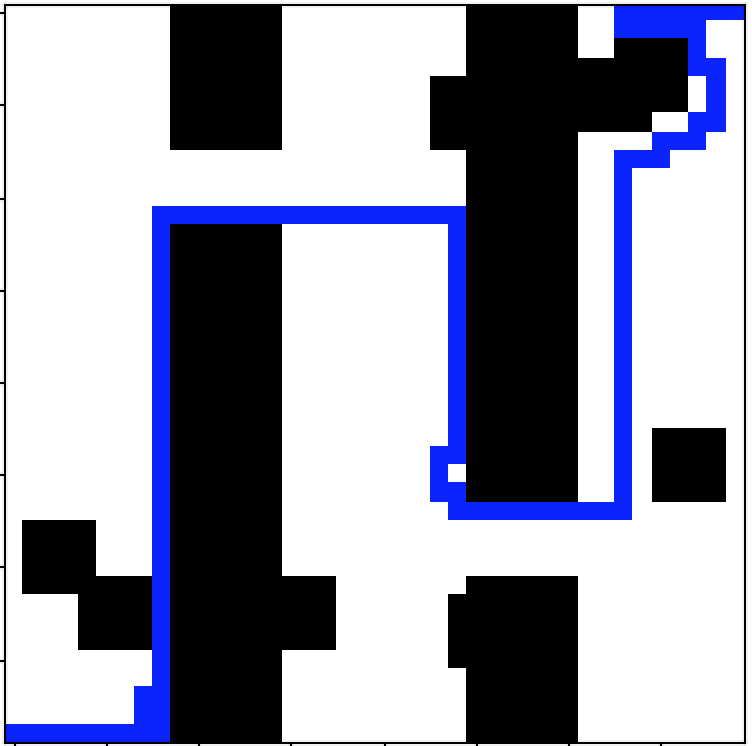
\includegraphics[width=.2\textwidth]{figures/add_conv.png}

\caption{We compare the solutions of \phil trained with a GAT (left), DeeperGCN (\textit{softmax}) (middle), and MPNN (\textit{sum}) (right). Results demonstrate that MPNN (\textit{sum}) makes several redundant expansions while the other two methods expand paths close to optimally.}
\label{fig:figure-3convs}
\end{figure}

\paragraph{Conclusion} The GNN ablation demonstrates that maximisation-based aggregation performs better, with an average reduction of explored nodes by $1.57 \%$. This finding is consistent with Veličković \etal \cite{velivckovic2019neural}, where GNNs are applied to execute graph algorithms. While the problem solved by  Veličković \etal \cite{velivckovic2019neural} is different, its nature is similar: train a GNN to \textit{select} which node to explore next in order to imitate a reference graph algorithm. In \phil, scores are assigned to nodes rather than nodes being selected, but the downstream operation is node selection. Further, these experiments also suggest that attention can be helpful in more complex graphs, with GAT outperforming other approaches in the \textit{Gaps+Forest} graphs.

\subsection{Increasing neighborhood size} As explained in the approach (Section \ref{sec:approach}), for each new fringe node we uniformly sample an $n \in \mathbb{N}_{\geq 0}$ bounded neighborhood of nodes, which we then use for graph convolutions. We hypothesized that with increasing $n$, the performance of \phil will improve. In Figure \ref{fig:sampling_extent}, we validate this hypothesis on \textit{Alternating gaps}, \textit{Forest}, and \textit{Gaps+Forest} datasets, by gradually setting $n = 0, 1, 2, 4$. We train \phil using a DeeperGCN (\textit{softmax}) graph convolution, $t_\tau = 16$, and with otherwise the same set of hyperparameters as in the \textit{Zeroed-out states vs. Rolled-in states} (Appendix \ref{sec:zeronero}) experiment. In Figure \ref{fig:sampling_extent}, we report the explored node ratio of each method with respect to the optimal number of explored nodes, that is, the shortest paths between start \& goal pairs.


\begin{figure}[htpb]
\centering
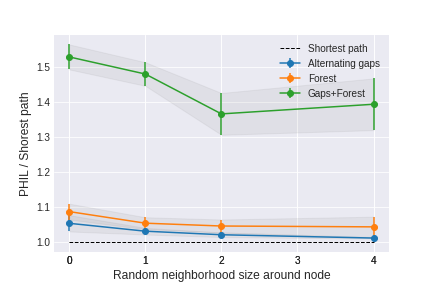
\includegraphics[width=0.6\textwidth]{figures/neighbors.png}
\caption{This plot illustrates the performance of \phil with increasing $n = |\mathcal{N}_i|$ through $0, 1, 2, 4$ for each evaluated fringe node $i$.}
\label{fig:sampling_extent}
\end{figure}

\paragraph{Conclusion} In Figure \ref{fig:sampling_extent}, we may observe that on all datasets the performance of \phil improves with increasing $n = |\mathcal{N}_i|$ until $n = 2$, after which it plateaus. These results suggest that \phil can benefit from additional nodes sampled from the neighbourhoods of evaluated fringe nodes, even if this sampling is performed uniformly at random.


\subsection{Increasing memory capacity}

In the final ablation experiment, we consider what effects changing the capacity of memory ($d$) has on the overall performance of \phil. We alter $d = 1, 16, 32, 64, 128, 256$ across all datasets. In Figure \ref{fig:memory_capacity}, the ratio of explored nodes is presented with respect to the shortest path length, which is the optimal baseline.

Focusing on the \textit{Gaps+Forest} dataset, in Figure \ref{fig:memory_capacity} we can observe that the performance of \phil generally improves until about $d = 32$ by approximately $40 \%$ with respect to $d=1$, after which it starts getting worse. Hence, we can conclude that additional memory capacity can be helpful for \phil to learn representations better suited for inferring distances of newly added fringe nodes. Note that we trained \phil for a fixed number of iterations ($N = 36$) in all cases, which means that the decrease in performance after $d = 32$ could also be due to the $\textsc{GRU}$ module having more parameters to optimise, which may take longer to converge. However, it could also easily be that the memory module starts overfitting to samples in the aggregated dataset during training. In the case of the simpler \textit{Alternating gaps} and \textit{Forest} datasets, the differences between different amounts of memory capacity are marginal. These findings are supported by approaches such as \sail \cite{bhardwaj2017learning} achieving good performances in simpler environments. By implication, performance decrease in the \textit{Gaps+Forest} dataset for larger values of $d$ is more likely due to overfitting than optimisation difficulties.


\begin{figure}[!htpb]
\centering
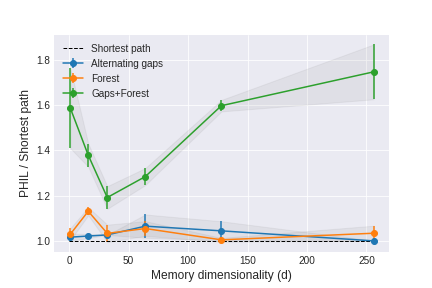
\includegraphics[width=0.6\textwidth]{figures/memory_capacity.png}
\caption{This plot illustrates the performance of \phil with increasing $d$ through $1, 16, 32, 64, 128, 256$ on the three ablation datasets.}
\label{fig:memory_capacity}
\end{figure}


\paragraph{Conclusion} Additional memory capacity is crucial for \phil to learn useful representations in more challenging graphs, while the importance of additional memory decreases as the graphs are simpler. However, a certain amount of overfitting is observed for larger values of $d$, which means that $d$ should be tuned on a per problem basis.


\newpage
\section{Architecture}

\begin{figure}[!htpb]
    \centering
    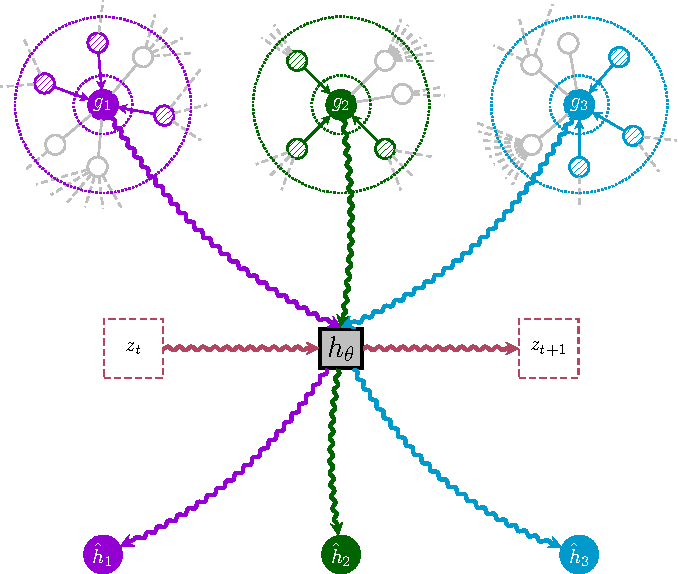
\includegraphics[width=0.75\textwidth]{figures/model.pdf}
    \caption{This figure illustrates the computation performed in a single forward pass of $h_\theta$. In the case of this figure, we would have $|\VS_{new}| = n = 3$, with $g_i$ representing the convolved embeddings, and $\hat{h}_i$ the output heuristic values. Horizontally, we illustrate the update of memory $z_t$ to $z_{t+1}$. This figure is adapted from \cite{figurespetar}.
    }
    \label{fig:inference}
\end{figure}



\section{Qualitative Examples}
\begin{figure}[!htpb]
    \centering
    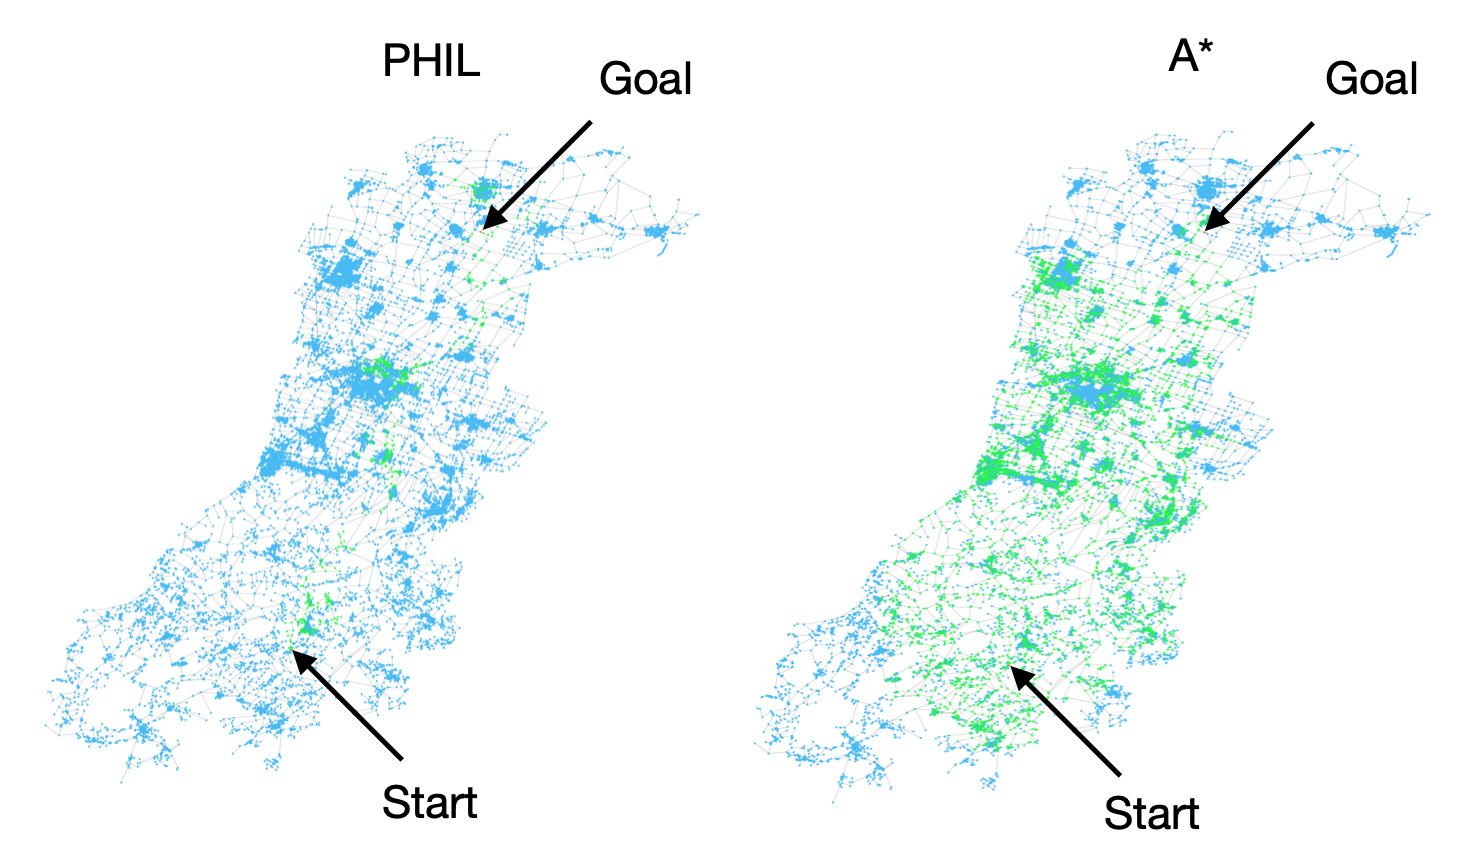
\includegraphics[width=0.9\columnwidth]{figures/comp_modena.png}
    \caption{This figure illustrates the road network of Modena, Italy. We contrast the search effort of \phil (left) and A* (right). We can observe that \phil expands (shown in green) considerably fewer nodes searching for the goal $v_g$.}
    \label{fig:modena}
\end{figure}

\begin{figure}[!htpb]
    \centering
    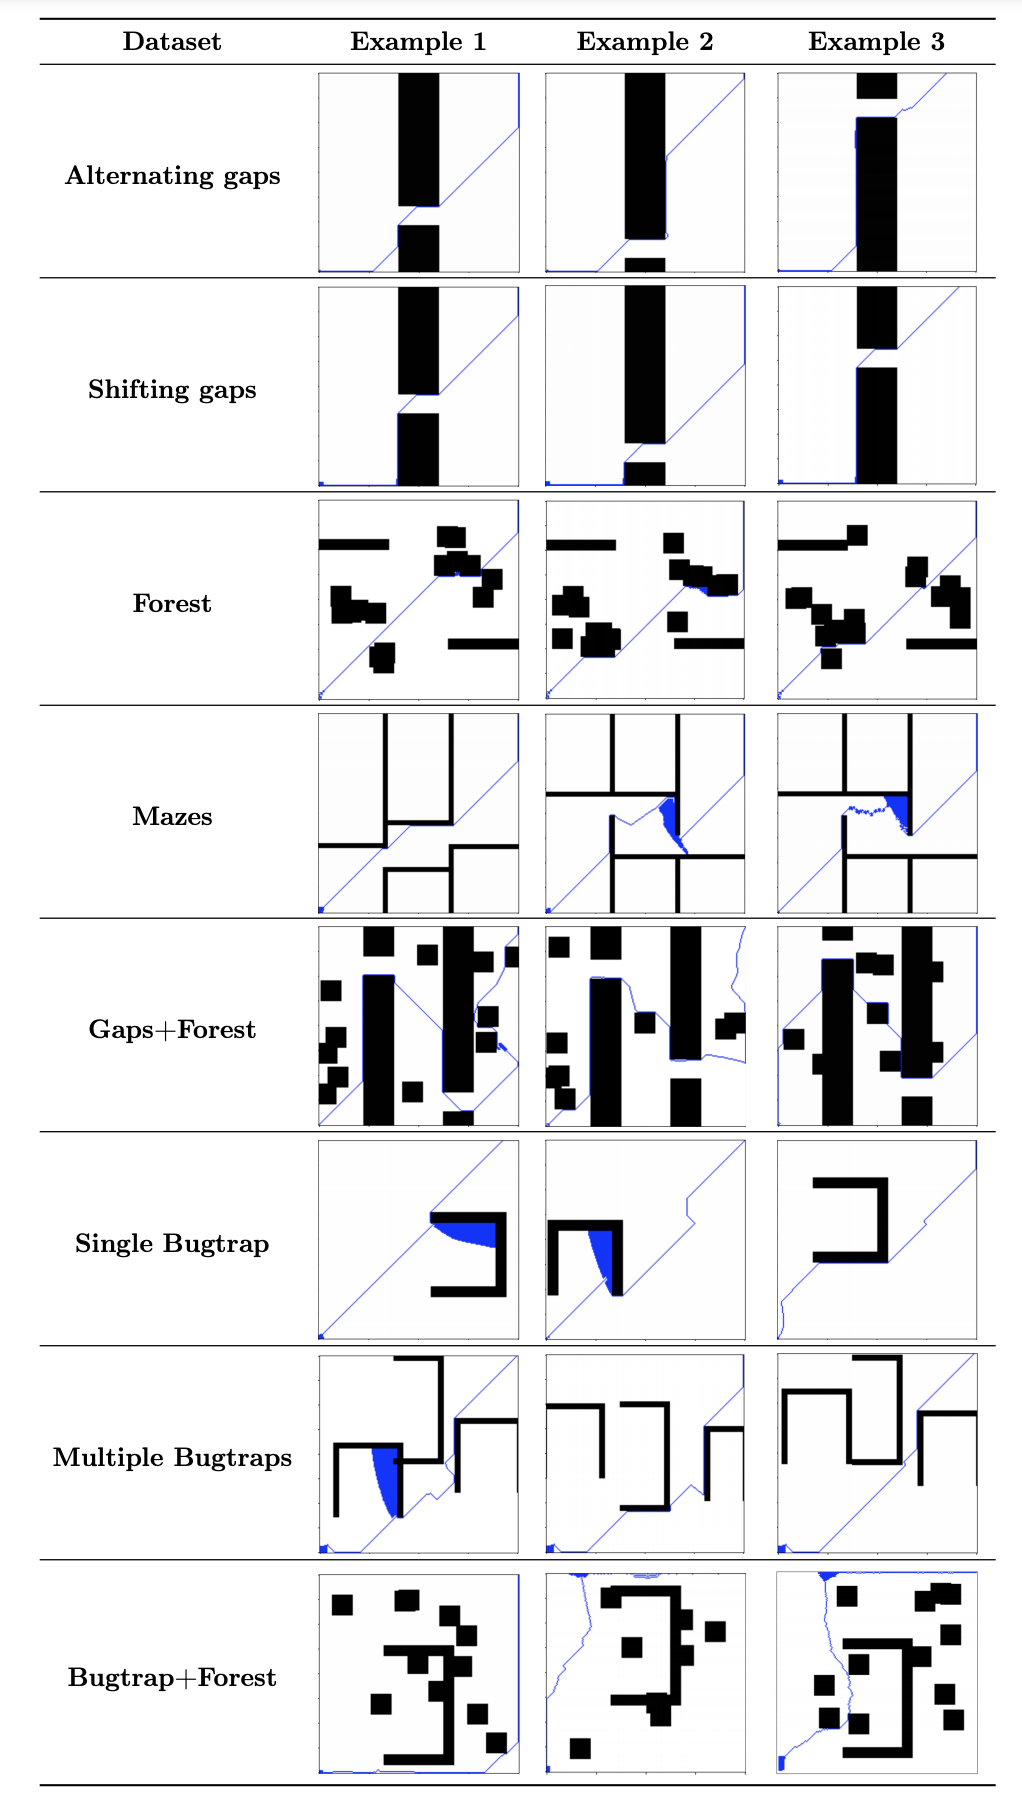
\includegraphics[width=0.9\columnwidth]{figures/grid.png}
    \caption{This figure presents representative examples of \phil runs in datasets from Section \ref{sec:experiments-grids}}
    \label{fig:grid}
\end{figure}



\end{document}
